
% ===============================================================
%
% For tracking purposes - this is V2.0 - May 2012

%\documentclass[acmlarge]{acmart}
\documentclass[10pt]{article}
\hoffset -1in \voffset -0.7in \textwidth 485pt \textheight 680pt



\usepackage{graphicx,epsfig,amsmath,amsthm,amssymb}
\usepackage{enumerate}
\usepackage{multirow}
\usepackage{bbm}
\usepackage{balance}
\usepackage{footnote}
\usepackage{tablefootnote}
\usepackage{xr}


\newtheorem{definition}{Definition}
\newtheorem{lemma}{Lemma}
\newtheorem{clm}{Claim}
\newtheorem{proposition}{Proposition}
\newtheorem{assumption}{Assumption}
\newtheorem{theorem}{Theorem}
\newtheorem{corollary}{Corollary}
\newtheorem{example}{Example}
\newtheorem{remark}{Remark}

\begin{document}




\title{The title of your project}  %
\author{Your name and project group}

\maketitle


\section{Introduction}
Introduce your problem here. Key elements in this section are: 
\begin{enumerate}
	\item In this report, we focus on the problem of...
	\item The importance and main contributions of this report.
\end{enumerate}

\section{Model and Problem Statement}
You can either use mathematical formulas as follows
\begin{equation}
\label{op}
\begin{array}{l}
\mathop {\max }\limits_{({P_{s,1}}, {P_{s,2}}, {P_r}, {\omega _r}, {\omega _t})} EE\\
s.t.\left\{ \begin{array}{l}
R_{\mathrm{sum}}  \ge R_{\min}\\
1 \le \left| {{\omega _r}} \right| =  \left| {{\omega _t}} \right| \le {N_r}\\
0 < {P_r} \le P_r^{\max }, 0 < {P_{s,k}} \le P_s^{\max }, k \in \{1,2\}.
\end{array} \right.
\end{array}
\end{equation}

Or, you should have a clear description of your problem in details.

Then, you can end this section with the main challenges behind your problem.

\section{Main Results}
In this section, you should compared different possible solutions found in the literature \cite{zhou2015energy}~\cite{zhou2014energy}, and discuss their advantages or disadvantages in your scenarios. Then, you should try to choose one of them to go depth in the following. Or you can propose your own solution by combining previous ones or improve previous ones. If possible, you might try to prove something, and state it in a theorem or proposition as follows.
\begin{theorem}
	$\sqrt{2}$ is an irrational number.
\end{theorem}
\begin{proof}
	We will prove this by contradiction.
\end{proof}
\begin{proposition}
	Consider an M/M/1 system with arrival rate $\lambda$ and service rate $\mu$, the average response time is $\frac{1}{\mu-\lambda}$.
\end{proposition}


\section{Numerical Results}
In this section, if possible (bonus points!), you can use simulations (for example, via Matlab, Python) to demonstrate the performance of your solution. Or, you should at least consider using the results in the papers you surveyed. Remember, you should not just copy them here. Rather, you should describe and explain the results.

\begin{figure}[t]
\centering
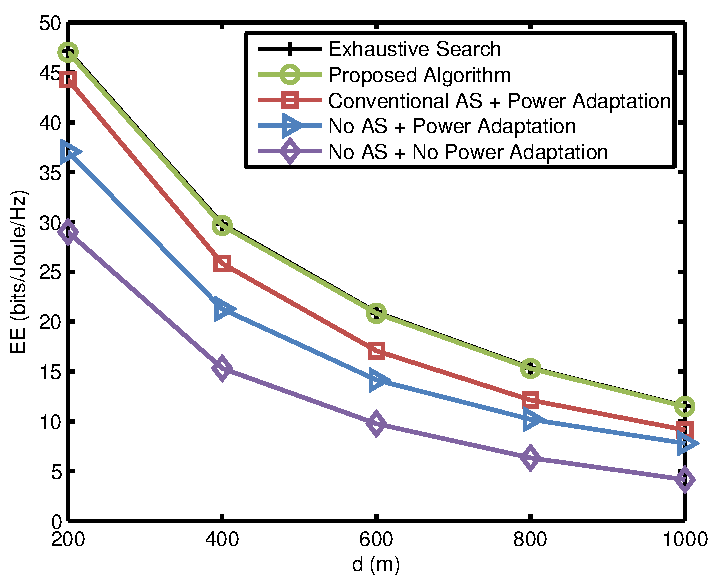
\includegraphics[width=3.5in]{Fig_EE_color.pdf}
\caption{Energy efficiency VS. the  distance $d$ with $\varepsilon = 0.5$ \label{fig:EE}}
\end{figure}

\section{Discussion}
In this section, you might talk some generalizations or extensions of your solution.

\section{Group Dynamics}
Summarize the group work so far.

\section{Conclusion}
Conclude your problem in a short paragraph.



\bibliographystyle{plain}
\bibliography{ref}
\appendix
\section{Code Appendix}
In the appendix, you can provide further materials such as codes and additional simulation results.





\end{document}
